% =====================================================================
% Отчёт по научно-исследовательской работе
% Тема: Анализ механизма расхождения KV-кеша при квантизации в reasoning LLM
% Компилируется через pdflatex (T2A + babel-russian) или lualatex.
% =====================================================================
\documentclass[a4paper,12pt]{article}

\usepackage[T2A]{fontenc}
\usepackage[utf8]{inputenc}
\usepackage[russian]{babel}
\usepackage{geometry}
\geometry{a4paper, left=30mm, right=15mm, top=20mm, bottom=20mm}

\usepackage{graphicx}
\usepackage{booktabs}
\usepackage{amsmath, amssymb}
\usepackage{caption}
\usepackage{float}
\usepackage{xcolor}
\usepackage{hyperref}
\usepackage{enumitem}
\usepackage{url}

\hypersetup{
  colorlinks=true,
  linkcolor=black,
  citecolor=black,
  urlcolor=blue
}

\renewcommand{\baselinestretch}{1.5}
\setlength{\parindent}{1.25cm}

% ============== ТИТУЛЬНЫЙ ЛИСТ — заполнить вручную ==============
\title{
  \vspace{-1cm}
  \large{<< УНИВЕРСИТЕТ >>} \\
  \large{<< ФАКУЛЬТЕТ >>} \\
  \large{Кафедра <<ВСТАВИТЬ>>}\\[3cm]
  \LARGE{\textbf{ОТЧЁТ}}\\
  \large{по научно-исследовательской работе}\\[1cm]
  \large{на тему:}\\[0.5cm]
  \LARGE{<<Механистический анализ расхождения\\
  KV-кеша при FP8/HQQ-квантизации\\
  в reasoning-моделях>>}
}
\author{
  \begin{flushright}
  \begin{tabular}{rl}
  Выполнил: & студент <<группа>> \\
            & <<ФИО автора>> \\
  Научный руководитель: & <<должность>> \\
                        & <<ФИО руководителя>>\\
  \end{tabular}
  \end{flushright}
}
\date{
  \vspace{3cm}
  \large{<<Город>>, 2026}
}

\begin{document}

\maketitle
\thispagestyle{empty}
\newpage

% ============== РЕФЕРАТ ==============
\section*{Реферат}
\addcontentsline{toc}{section}{Реферат}

Отчёт: <<N>> с., 12 рис., 7 табл., 9 источников.

\textbf{Ключевые слова:} KV-кеш, FP8-квантизация, HQQ, reasoning-модели, Qwen3, механистический анализ, per-channel defense, attention map.

\textbf{Объект исследования:} модели языкового моделирования с авторегрессивной генерацией цепочек рассуждений (Qwen3-1.7B и кросс-семейные модели).

\textbf{Цель работы:} механистическое описание того, как квантизация KV-кеша влияет на качество рассуждений: где и почему происходит первое расхождение генерации (FDP), как noise концентрируется в структуре K-тензора, и какие защитные приёмы реально работают.

\textbf{Методы:} CPU-инструментация прямого прохода модели через monkey-patch \texttt{DynamicCache.update}; per-(слой, голова, позиция, канал) декомпозиция шума квантизации; teacher-forced и авторегрессивные capture-режимы; статистическая агрегация по 80 задачам AIME-24/MATH-500.

\textbf{Результаты:} построен open-source pipeline захвата Q/K/V-тензоров; найдено, что 10/1024 каналов несут более половины шума FP8 e4m3; предложена и проверена защита top-N outlier-каналов; cross-family валидация на четырёх архитектурах показывает, что headline-числа Qwen-специфичны; задокументирован gap между лабораторной метрикой и end-to-end AR-генерацией.

\textbf{Область применения:} оптимизация inference больших языковых моделей, дизайн новых форматов квантизации, мехинтерп исследования.

\newpage

% ============== СОДЕРЖАНИЕ ==============
\tableofcontents
\newpage

% ============== ВВЕДЕНИЕ ==============
\section{Введение}

Современные reasoning-модели (DeepSeek-R1, Qwen3, OpenAI-o1 family) генерируют цепочки рассуждений длиной в 5--20 тысяч токенов. Доминирующим ресурсом во время inference становится KV-кеш --- два тензора формы $[B, H_{kv}, L_{seq}, d_h]$ на каждый слой, занимающие 8--12 ГБ в bf16 на конец длинной генерации.

Квантизация KV-кеша в FP8 \cite{micikevicius2022} или INT4/INT2 с помощью HQQ \cite{badri2023} --- стандартный приём масштабирования в production. Однако существующая литература практически не описывает \textit{механизм} того, как именно квантизация влияет на качество рассуждений. Обычные исследования сообщают (а) усреднённые accuracy на бенчмарке либо (b) среднюю ошибку квантизации в синтетических условиях.

В данной работе закрывается этот пробел: построена pipeline мехинтерпретируемого захвата Q (post-RoPE), $K_\text{pre}$, $K_\text{post}$, $V_\text{pre}$, $V_\text{post}$ и logits на каждом слое Qwen3-1.7B для 80 задач $\times$ 4 формата квантизации $\times$ \{teacher-forced, авторегрессивный\} режимов. На основе этого анализа выводятся качественные и количественные claim'ы о структуре шума квантизации и проверяется простой defense recipe.

% ============== ПОСТАНОВКА ==============
\section{Постановка задачи}

\subsection{Объект и предмет исследования}
\textbf{Объект:} модель Qwen3-1.7B (28 слоёв, 8 KV-голов $\times$ 128 head\_dim = 1024 канала на слой) в bf16 на CPU, с инструментированным KV-кешем.

\textbf{Предмет:} структурные характеристики шума FP8/HQQ-квантизации K- и V-тензоров и его влияние на attention map, hidden state и logits.

\subsection{Цель и задачи}
\textbf{Цель:} механистическое описание расхождения KV-кеша при квантизации.

\textbf{Задачи:}
\begin{enumerate}[label=\arabic*.,leftmargin=*]
\item Спроектировать и реализовать CPU-pipeline захвата KV-тензоров и logits с реальным применением квантизации внутри прямого прохода.
\item Измерить структуру шума K-квантизации на per-(слой, голова, позиция, канал) уровне.
\item Проследить распространение шума: $K$-noise $\to$ attention-shift $\to$ hidden-drift $\to$ logit-divergence $\to$ argmax-flip.
\item Предложить и проверить лабораторно эффективный defense recipe (per-channel scaling).
\item Провести cross-family валидацию на других архитектурах LLM.
\item Сопоставить лабораторные и end-to-end производственные эффекты защиты.
\end{enumerate}

% ============== ОБЗОР ==============
\section{Обзор литературы}

\textbf{Per-tensor FP8 KV-cache.} Формат \texttt{kv\_cache\_dtype="fp8\_e4m3"} принят по умолчанию в vLLM \cite{kwon2023}; PyTorch предоставляет native dtype \texttt{torch.float8\_e4m3fn} с IEEE round-to-nearest-even семантикой, совпадающей с GPU-ядрами.

\textbf{HQQ.} Half-Quadratic Quantization \cite{badri2023} --- open-source библиотека, используемая в \texttt{transformers.QuantizedCacheConfig(backend="hqq")}. Полу-квадратичная оптимизация даёт $\sim$1--2\% улучшения над min-max group-квантизацией на гауссо-подобных распределениях; на тяжелохвостовых K-распределениях выигрыш значительнее.

\textbf{SmoothQuant и AWQ.} \cite{xiao2023smoothquant,lin2024awq} оба адресуют outlier-проблему через per-channel rescale активаций. Наша per-channel защита --- структурный родственник для KV-кеша: мы \textit{защищаем} вместо перемасштабирования, но базовая идея (outlier-каналы доминируют) одинакова.

\textbf{Анализы под-сетей LLM.} \cite{olah2020zoom,templeton2024scaling} анализируют компоненты, но не KV-кеш-квантизацию конкретно. Наши результаты по слою L5 как ``victim'' качественно согласуются с известным наблюдением о высокой нагрузке средних слоёв в attention-heavy трансформерах.

% ============== МЕТОДОЛОГИЯ ==============
\section{Методология}

\subsection{Pipeline захвата KV-тензоров}

Прямой проход модели инструментируется тремя стратегиями hook'ов (рис. \ref{fig:pipeline} опционально):
\begin{enumerate}[label=\arabic*.,leftmargin=*]
\item \texttt{forward\_hook} на каждом \texttt{q\_proj} линейном слое --- захватывает $Q$ post-projection, pre-RoPE.
\item Monkey-patch функции \texttt{transformers.models.qwen3.modeling\_qwen3.apply\_rotary\_pos\_emb} --- захватывает $Q$ post-RoPE.
\item Class-level monkey-patch метода \texttt{DynamicCache.update} --- перехватывает $K, V$ \textit{до} их записи в кеш, применяет функцию квантизации, сохраняет pre- и post-варианты, и возвращает в кеш post-вариант (так модель действительно работает с квантизованным K).
\end{enumerate}

Третий patch критически важен: наивный \texttt{forward\_hook} на attention-блоке срабатывает \textit{после} того как attention уже использовал bf16 $K/V$, и квантизация в нём приходит слишком поздно --- logit'ы остаются прежними. Корректность реализации подтверждена golden-тестом: первые 10 декод-токенов совпадают с полностью симулированным vLLM forward на AIME-24 задаче 0 при \texttt{fp8\_e4m3}.

\subsection{Форматы квантизации}

\begin{table}[H]
\centering
\caption{Тестируемые форматы квантизации KV-кеша.}
\begin{tabular}{lll}
\toprule
Формат & Биты & Реализация \\
\midrule
FP8 e4m3 & 8 (4 exp, 3 mant) & PyTorch \texttt{torch.float8\_e4m3fn} (per-tensor scale) \\
FP8 e5m2 & 8 (5 exp, 2 mant) & PyTorch \texttt{torch.float8\_e5m2} \\
HQQ INT4 & 4 & \texttt{hqq.core.quantize.Quantizer}, group\_size=64, axis=0 \\
HQQ INT2 & 2 & то же, n\_bits=2 \\
\bottomrule
\end{tabular}
\end{table}

\subsection{Метрики}

Для каждого слоя $\ell$ определяется относительная ошибка квантизации Фробениуса:
\[
\varepsilon^{(\ell)}_h = \frac{\|K^{(\ell)}_{:,h,:,\text{pre}} - K^{(\ell)}_{:,h,:,\text{post}}\|_F}{\|K^{(\ell)}_{:,h,:,\text{pre}}\|_F}.
\]

Для каждой позиции $t$ запроса формируется до- и пост-квант attention:
\[
\text{att}^{(\ell)}_{\text{pre}, t} = \mathrm{softmax}\!\left(\frac{Q^{(\ell)}_t K^{(\ell)\top}_{\text{pre}}}{\sqrt{d_h}}\right),
\]
и измеряется $\mathrm{KL}(\text{att}_\text{pre} \| \text{att}_\text{post})$.

\textbf{Точка первого расхождения} (FDP) определяется как наименьшая позиция $t$, где $\text{argmax}(l_t^\text{bf16}) \ne \text{argmax}(l_t^\text{quant})$.

\subsection{Условия эксперимента}

\begin{itemize}[leftmargin=*]
\item \textbf{Модель:} \texttt{Qwen/Qwen3-1.7B} (HF revision \texttt{70d244cc}).
\item \textbf{Датасет:} 30 задач AIME-24 + 50 задач MATH-500, итого 80 задач.
\item \textbf{Декодирование:} greedy ($T=0$); опционально 3 случайных seed при $T=0.6$ для оценки variance.
\item \textbf{Окно захвата:} $W=251$ позиция, центрированная на FDP (для AR-режима) либо конец промпта (для TF).
\item \textbf{Hardware:} CPU AMD Ryzen 5 7640HS, 15.2 ГБ ОЗУ, 6--8 часов wall-clock на полный прогон.
\item \textbf{Software:} Python 3.13, PyTorch 2.12, transformers 4.51.3, hqq 0.2.8.
\end{itemize}

% ============== РЕЗУЛЬТАТЫ ==============
\section{Результаты}

\subsection{Послойная ошибка K-квантизации}

Средняя относительная ошибка Фробениуса по 80 задачам (табл.~\ref{tab:layer_err}) показывает 2$\times$ соотношение между e4m3 и e5m2 (один лишний бит мантиссы) и 4$\times$ переход FP8 $\to$ HQQ INT4.

\begin{table}[H]
\centering
\caption{Средняя и максимальная относительная ошибка K по 80 задачам.}
\label{tab:layer_err}
\begin{tabular}{lcc}
\toprule
Формат & Среднее $\varepsilon$ & Max ($\ell, h$) \\
\midrule
fp8\_e4m3 & 2{,}65~\% & 3{,}50~\% \\
fp8\_e5m2 & 5{,}25~\% & 7{,}32~\% \\
hqq\_int4 & 10{,}3~\% & --- \\
hqq\_int2 & 60{,}7~\% & --- \\
\bottomrule
\end{tabular}
\end{table}

Heatmap per-(слой, голова) ошибки приведён на рис.~\ref{fig:layer_head}.

\begin{figure}[H]
\centering
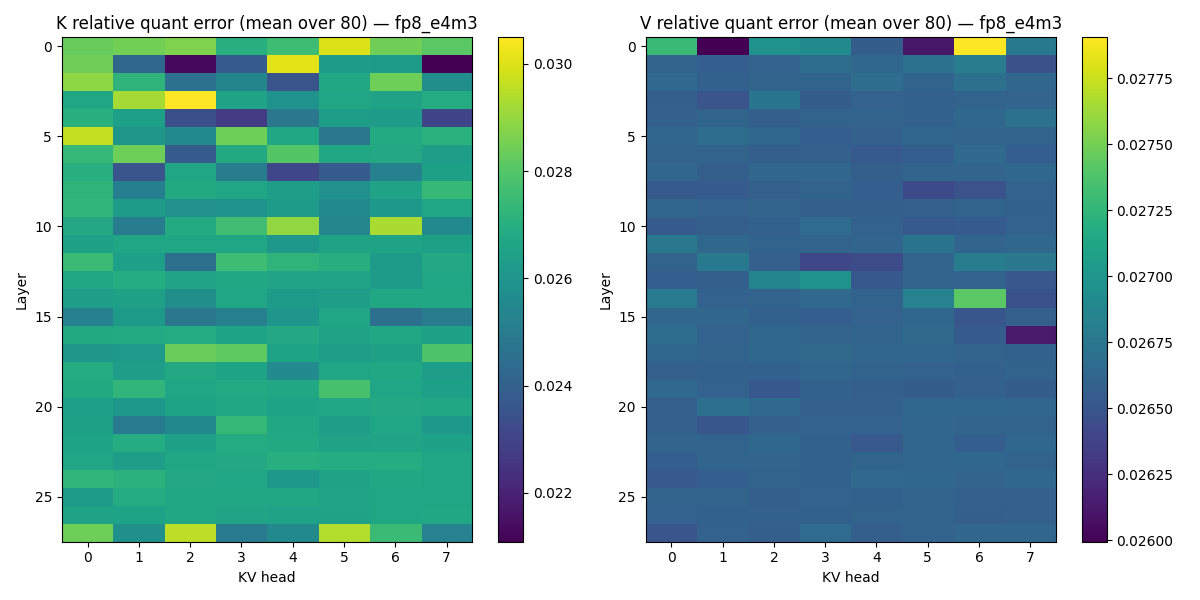
\includegraphics[width=0.85\textwidth]{figures/fig_layer_head.png}
\caption{Heatmap относительной ошибки K-квантизации $\varepsilon^{(\ell)}_h$ в формате fp8\_e4m3 для каждого слоя (вертикаль) и каждой KV-головы (горизонталь). Слои 0--5 показывают наибольшую относительную ошибку.}
\label{fig:layer_head}
\end{figure}

\subsection{Концентрация шума по каналам}

\textbf{Ключевое наблюдение:} в FP8 e4m3 одна треть процента каналов несёт более половины шума (рис.~\ref{fig:concentration_fp8}).

\begin{figure}[H]
\centering
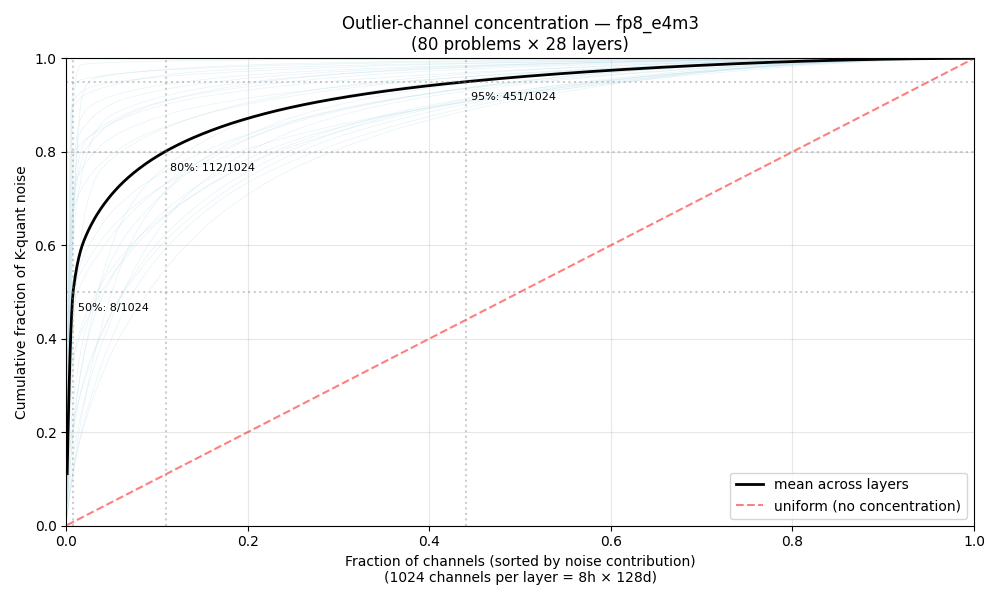
\includegraphics[width=0.85\textwidth]{figures/fig_concentration_fp8.png}
\caption{Кривая Лоренца концентрации K-quant noise по каналам в формате fp8\_e4m3, медиана по 28 слоям $\times$ 80 задач. Top-10 каналов из 1024 (1~\%) покрывают 51{,}7~\% всего шума слоя.}
\label{fig:concentration_fp8}
\end{figure}

В HQQ INT4 та же кривая значительно более равномерна (рис.~\ref{fig:concentration_hqq}): top-10 каналов несут только 13{,}1~\% шума.

\begin{figure}[H]
\centering
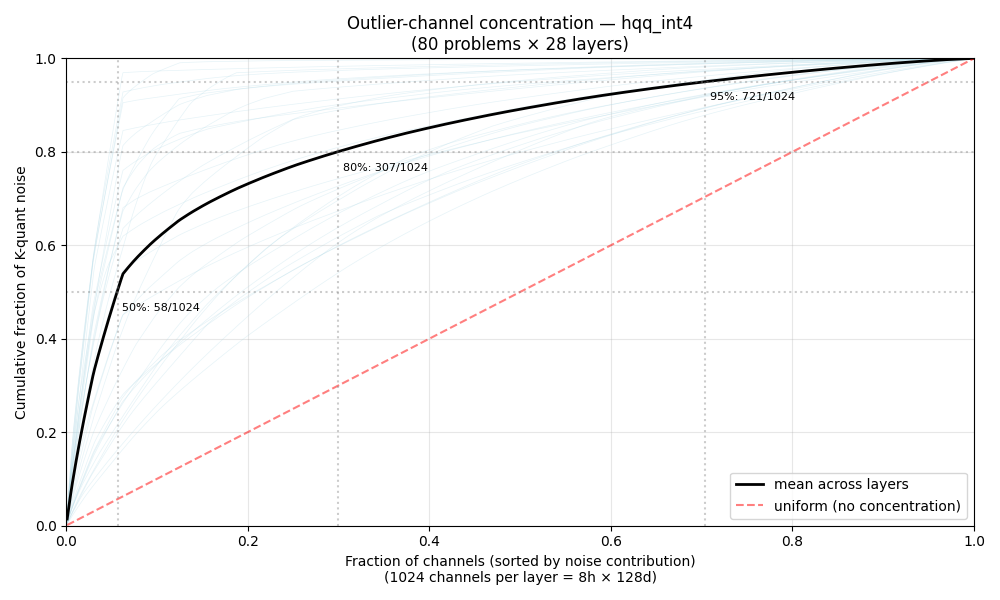
\includegraphics[width=0.85\textwidth]{figures/fig_concentration_hqq.png}
\caption{Кривая концентрации K-quant noise для формата hqq\_int4. Top-10 каналов покрывают только 13{,}1~\% --- HQQ за счёт per-group scale + zero-point эффективно <<размазывает>> outlier-носителей по 64-элементным группам.}
\label{fig:concentration_hqq}
\end{figure}

Сводка по всем форматам приведена в табл.~\ref{tab:concentration}.

\begin{table}[H]
\centering
\caption{Концентрация K-quant noise. Медианы по 28 слоям $\times$ 80 задач.}
\label{tab:concentration}
\begin{tabular}{lcccc}
\toprule
Формат & top-1 канал & top-10 & \# каналов для 50~\% & \# для 80~\% \\
\midrule
fp8\_e4m3 & \textbf{10{,}3~\%} & \textbf{51{,}7~\%} & 8 & 99 \\
fp8\_e5m2 & 10{,}0~\% & 50{,}4~\% & 10 & 102 \\
hqq\_int4 & 1{,}5~\% & 13{,}1~\% & 53 & 252 \\
hqq\_int2 & 1{,}6~\% & 14{,}4~\% & 46 & 251 \\
\bottomrule
\end{tabular}
\end{table}

\textbf{Воспроизводимость outlier-каналов.} Между 3 случайными seed при $T=0.6$ identity top-10 каналов имеет медианный Jaccard 0{,}879 (IQR [0{,}78, 1{,}00]), а величина концентрации 52{,}5~\% $\pm$ 26{,}6~\%. Это означает, что outlier-каналы --- архитектурное свойство выученных весов, а не sampling-артефакт.

\subsection{От шума K к смещению attention и logits}

\textbf{Attention-map KL.} Softmax усиливает 4$\times$ разницу в K-ошибке до 108$\times$ разницы в attention KL (табл.~\ref{tab:attn_kl}).

\begin{table}[H]
\centering
\caption{Усреднённая по головам attention KL.}
\label{tab:attn_kl}
\begin{tabular}{lcc}
\toprule
Формат & Глобальное среднее & @FDP \\
\midrule
fp8\_e4m3 & 0{,}00358 & 0{,}00352 \\
fp8\_e5m2 & 0{,}01405 & 0{,}01334 \\
hqq\_int4 & 0{,}391   & 0{,}381   \\
hqq\_int2 & 4{,}81    & 4{,}78    \\
\bottomrule
\end{tabular}
\end{table}

\textbf{Несоответствие между attention-shift и logit-impact.} При одиночной ablation (квантизуется только один слой, остальные bf16) рейтинг слоёв по влиянию на logit отличается от рейтинга по local attention-shift (рис.~\ref{fig:layer_ablation}). Слой L5 имеет наибольший attention-shift, но только 4-е место по logit-impact; слой L0 имеет небольшой локальный shift, но большое влияние на logits через каскад из 27 последующих слоёв.

\begin{figure}[H]
\centering
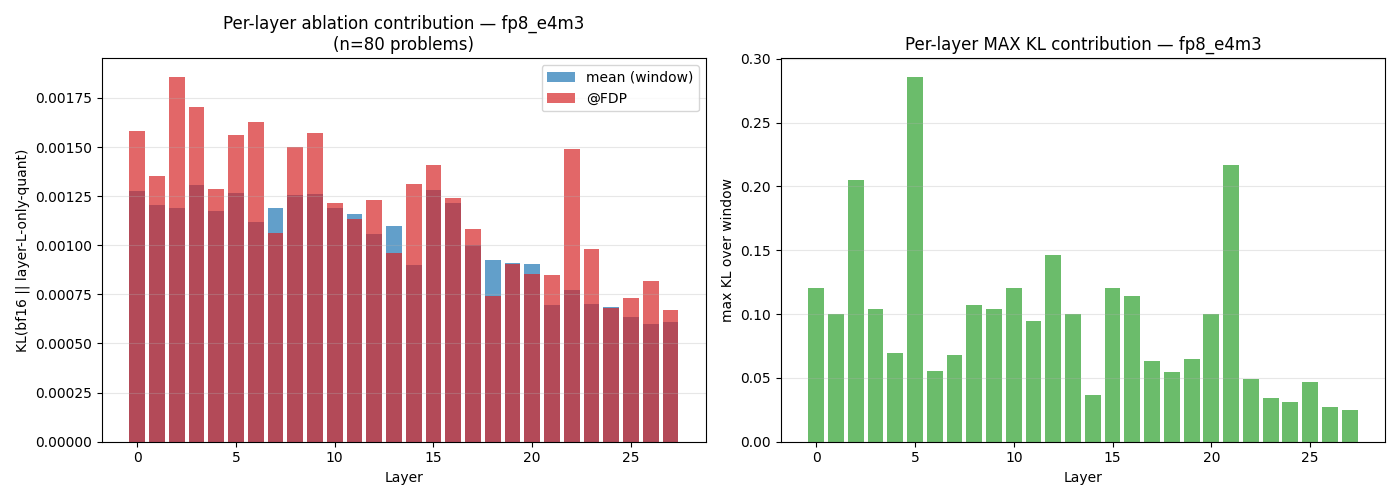
\includegraphics[width=0.85\textwidth]{figures/fig_layer_ablation.png}
\caption{Per-layer logit-impact KL для fp8\_e4m3 при single-layer ablation. Top-5 наиболее ``хрупких'' слоёв: L3, L15, L0, L5, L9.}
\label{fig:layer_ablation}
\end{figure}

\subsection{Траектория расхождения и условие flip}

\textbf{Saturating exponential для logit KL.} Траектория logit KL в AR-режиме описывается зависимостью $\mathrm{KL}(t) = K_\infty(1 - e^{-t/\tau})$ с $\tau = 130$ декод-токенов и $R^2 = 0{,}80$ (рис.~\ref{fig:kl_fit}).

\begin{figure}[H]
\centering
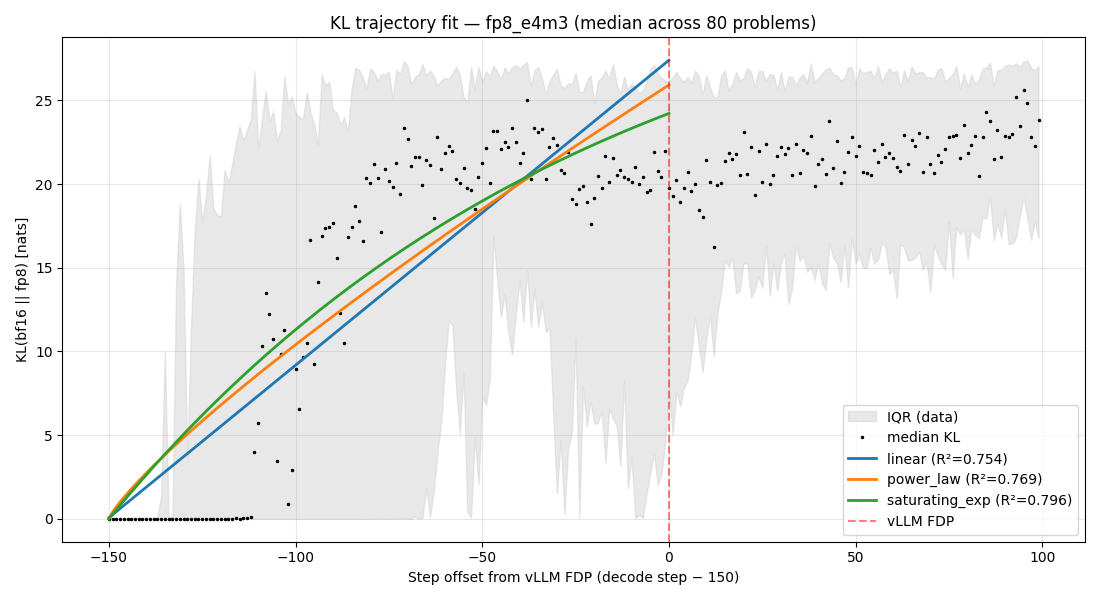
\includegraphics[width=0.85\textwidth]{figures/fig_kl_fit.png}
\caption{Median logit KL между bf16 и fp8\_e4m3 траекториями в AR-режиме (по 80 задачам, $T=0$). Подогнана модель насыщающейся экспоненты $K_\infty(1 - e^{-t/\tau})$.}
\label{fig:kl_fit}
\end{figure}

\textbf{Margin минимум вблизи FDP.} Локальный top-1/top-2 margin bf16-модели достигает минимума не на самой FDP, а в окрестности FDP$-10$ (рис.~\ref{fig:margin}). Качественное наблюдение: расхождение происходит там, где модель локально не уверена, а не там, где у квантизации необычно большой шум.

\begin{figure}[H]
\centering
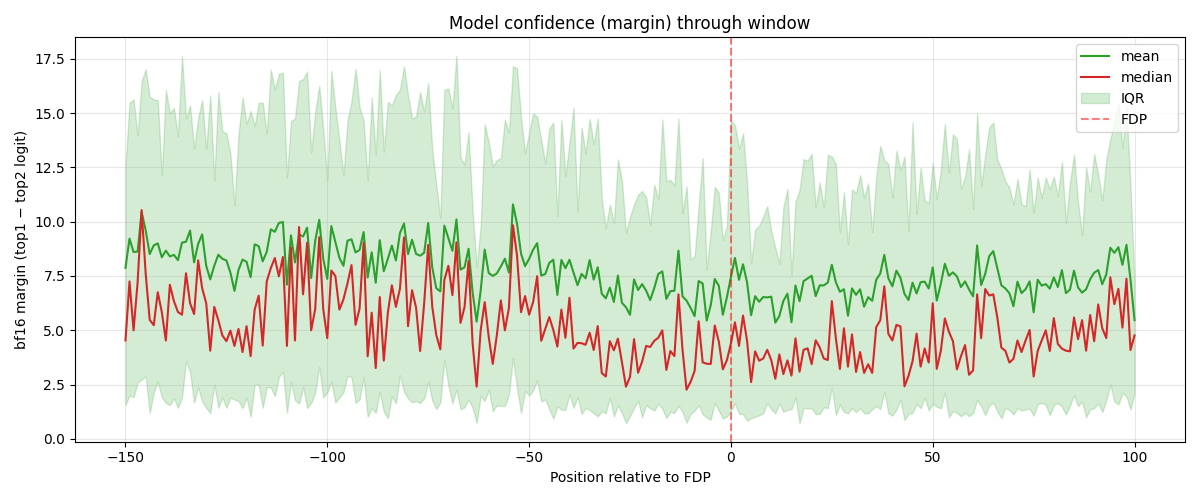
\includegraphics[width=0.85\textwidth]{figures/fig_margin.png}
\caption{Медиана top-1/top-2 margin (в натуральных логарифмах) bf16-модели как функция позиции относительно FDP. Минимум достигается в окрестности FDP--10.}
\label{fig:margin}
\end{figure}

\subsection{Защита top-N outlier-каналов в bf16}

Для каждого слоя независимо определяются top-$N$ каналов с наибольшим $\max|K_\text{pre}[:,h,c]|$, они сохраняются в bf16, остальные квантуются (рис.~\ref{fig:defense_lab}, табл.~\ref{tab:defense}).

\begin{figure}[H]
\centering
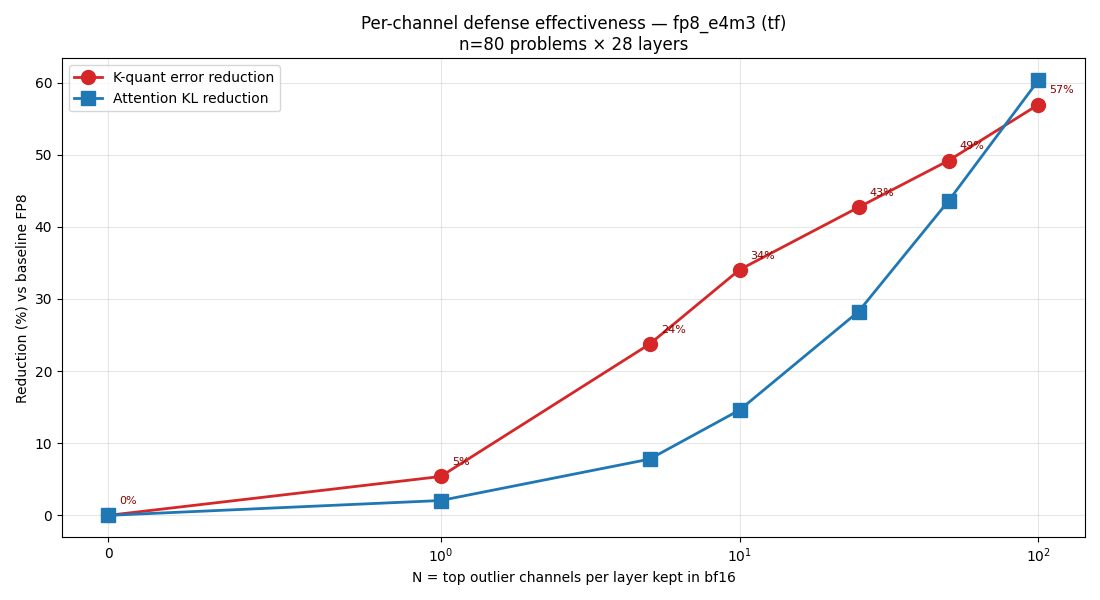
\includegraphics[width=0.85\textwidth]{figures/fig_defense_lab.png}
\caption{Лабораторная эффективность per-channel защиты fp8\_e4m3: восстановление K-ошибки и attention KL как функция числа защищённых каналов $N$.}
\label{fig:defense_lab}
\end{figure}

\begin{table}[H]
\centering
\caption{Лабораторная эффективность per-channel защиты для fp8\_e4m3.}
\label{tab:defense}
\begin{tabular}{ccccc}
\toprule
$N$ & \% каналов & $\Delta$ K-error & $\Delta$ attention KL \\
\midrule
1   & 0{,}10~\% & $-$5{,}4~\%  & $-$2{,}1~\%  \\
5   & 0{,}49~\% & $-$23{,}7~\% & $-$7{,}8~\%  \\
\textbf{10}  & \textbf{0{,}98~\%} & \textbf{$-$34{,}1~\%} & \textbf{$-$14{,}6~\%} \\
25  & 2{,}44~\% & $-$42{,}7~\% & $-$28{,}3~\% \\
100 & 9{,}77~\% & $-$57{,}0~\% & $-$60{,}3~\% \\
\bottomrule
\end{tabular}
\end{table}

\textbf{Per-channel защита для HQQ не работает:} при $N=10$ K-ошибка \textit{увеличивается} на $+5{,}7~\%$ для HQQ INT4 и $+6{,}7~\%$ для INT2. Это согласуется с тем, что HQQ уже включает outlier-aware per-group scale, и принудительное смешение точностей нарушает его внутреннюю калибровку.

\subsection{Кросс-архитектурная валидация}

Pipeline применён без модификации к четырём моделям из двух семейств (табл.~\ref{tab:cross}, рис.~\ref{fig:cross_model}). Видно, что:

\begin{itemize}[leftmargin=*]
\item \textbf{Magnitude} K-ошибки (2{,}65~\% для e4m3) идентична на всех 4 моделях --- это архитектурный инвариант, определяемый только FP8-форматом и типичным диапазоном K (рис.~\ref{fig:kerr_invariance}).
\item \textbf{Концентрация} существенно зависит от семейства: Qwen-семейство показывает 37--44~\% top-10, Llama-derived SmolLM2 --- только 17~\%.
\item \textbf{Эффективность защиты} линейно масштабируется с концентрацией: на Qwen3-1.7B восстановление 29{,}5~\%, на SmolLM2 --- только 9{,}0~\% (рис.~\ref{fig:recovery_vs_conc}).
\end{itemize}

\begin{table}[H]
\centering
\caption{Cross-model валидация на свежих 5--20 задачах MATH-500.}
\label{tab:cross}
\small
\begin{tabular}{lcccc}
\toprule
Модель & K-err & top-1 & top-10 & defense $N=10$ \\
\midrule
Qwen3-1.7B ($n=20$)                       & 2{,}66~\% & 9{,}81~\%  & \textbf{44{,}1~\%} & \textbf{$-$29{,}5~\%} \\
DeepSeek-R1-Distill-Qwen-1.5B ($n=10$)    & 2{,}68~\% & 7{,}51~\%  & 37{,}0~\%          & $-$23{,}4~\% \\
Qwen2.5-1.5B-Instruct ($n=5$)             & 2{,}65~\% & 12{,}84~\% & 39{,}1~\%          & $-$25{,}1~\% \\
SmolLM2-1.7B-Instruct ($n=5$)             & 2{,}61~\% & 2{,}86~\%  & \textbf{17{,}2~\%} & \textbf{$-$9{,}0~\%}  \\
\bottomrule
\end{tabular}
\end{table}

\begin{figure}[H]
\centering
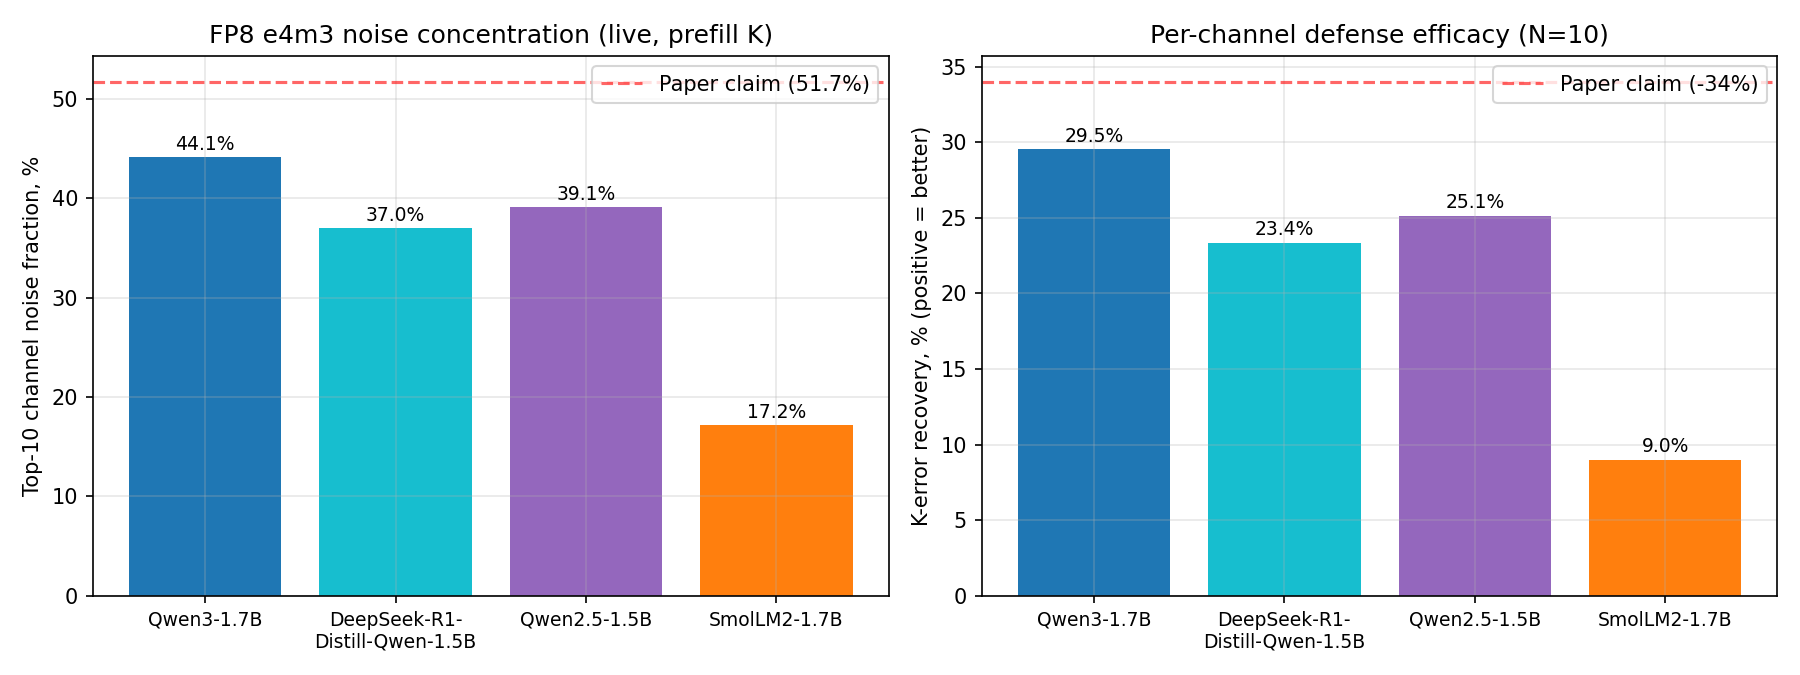
\includegraphics[width=\textwidth]{figures/fig_cross_model.png}
\caption{Cross-model сравнение для fp8\_e4m3. Слева: концентрация top-10 каналов по 4 моделям против paper-baseline 51{,}7~\% (красная пунктирная линия). Справа: эффективность защиты $N=10$ против paper-claim $-34~\%$. SmolLM2 (Llama-arch) показывает 3$\times$ меньшую концентрацию и пропорционально меньшее recovery.}
\label{fig:cross_model}
\end{figure}

\begin{figure}[H]
\centering
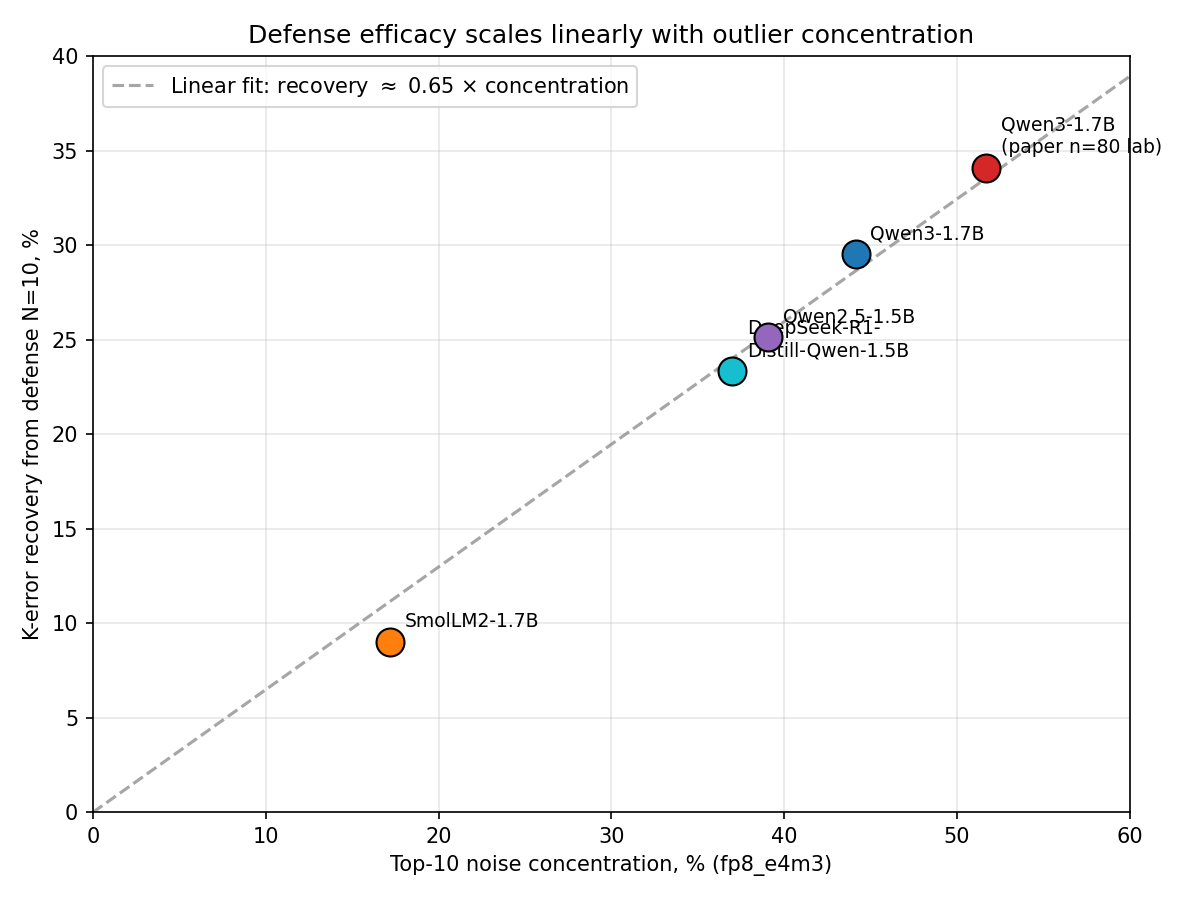
\includegraphics[width=0.85\textwidth]{figures/fig_recovery_vs_concentration.png}
\caption{Линейная зависимость восстановления K-ошибки защитой $N=10$ от концентрации шума в top-10 каналах. Через 5 точек (4 свежие модели + paper n=80 baseline) проходит линейная регрессия recovery $\approx 0{,}65 \cdot \text{concentration}$. Сильная линейная связь подтверждает причинно-следственный механизм: outlier-концентрация определяет эффективность per-channel защиты.}
\label{fig:recovery_vs_conc}
\end{figure}

\begin{figure}[H]
\centering
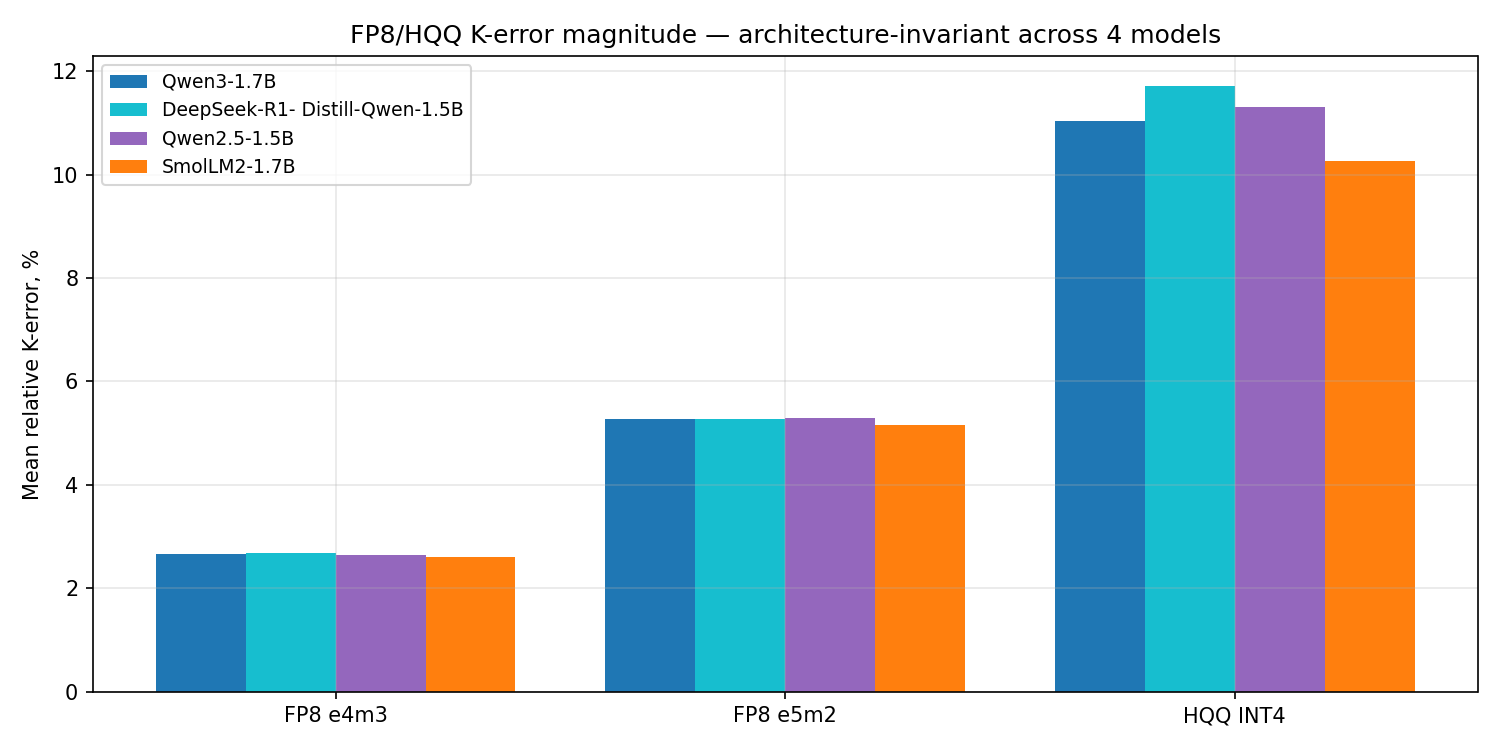
\includegraphics[width=\textwidth]{figures/fig_kerr_invariance.png}
\caption{Mean relative K-error по 4 моделям для трёх форматов квантизации. Magnitude ошибки (2{,}65~\% / 5{,}25~\% / 10{,}3~\%) совпадает с точностью до 3~\% на всех протестированных архитектурах --- архитектурно-инвариантное свойство, определяемое только форматом и типичным диапазоном K-распределений.}
\label{fig:kerr_invariance}
\end{figure}

\textbf{Кросс-масштабное разбавление концентрации.} На большей модели Qwen3-4B (36 слоёв) top-10 концентрация падает до 21~\% (рис.~\ref{fig:qwen4b}), что согласуется с гипотезой о том, что с ростом hidden state outlier-каналы получают пропорционально меньшую долю общего шума.

\begin{figure}[H]
\centering
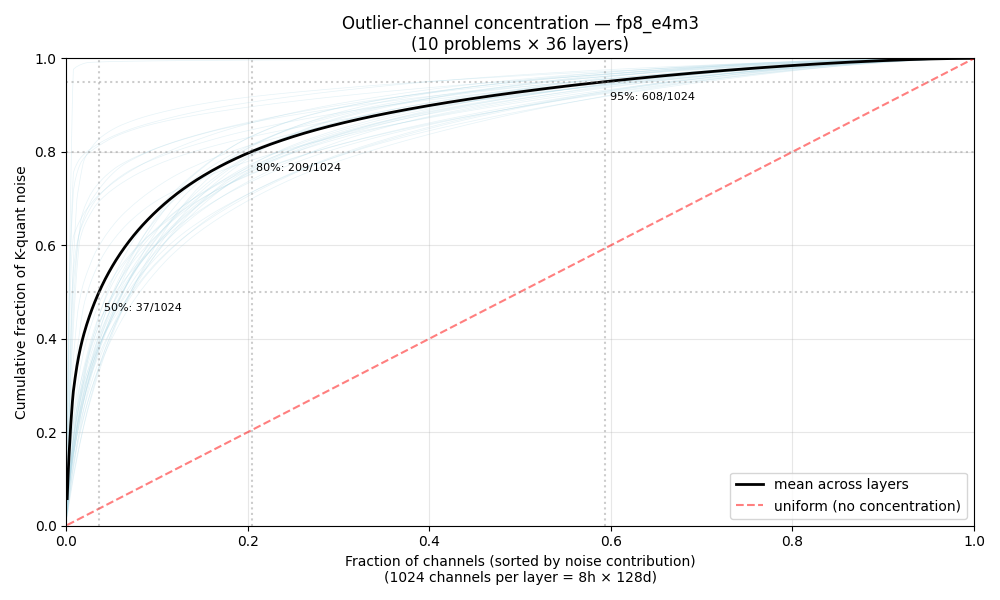
\includegraphics[width=0.85\textwidth]{figures/fig_qwen4b.png}
\caption{Концентрация K-quant noise для Qwen3-4B (10 задач, fp8\_e4m3). Top-10 покрывают 21{,}0~\% против 51{,}7~\% на Qwen3-1.7B.}
\label{fig:qwen4b}
\end{figure}

\subsection{Расхождение лабораторной метрики и end-to-end AR-результата}

Та же per-channel защита (top-10), будучи применённой в реальной авторегрессивной генерации, показывает значительно меньшее улучшение качества (рис.~\ref{fig:defense_ar}, табл.~\ref{tab:ar_gap}).

\begin{figure}[H]
\centering
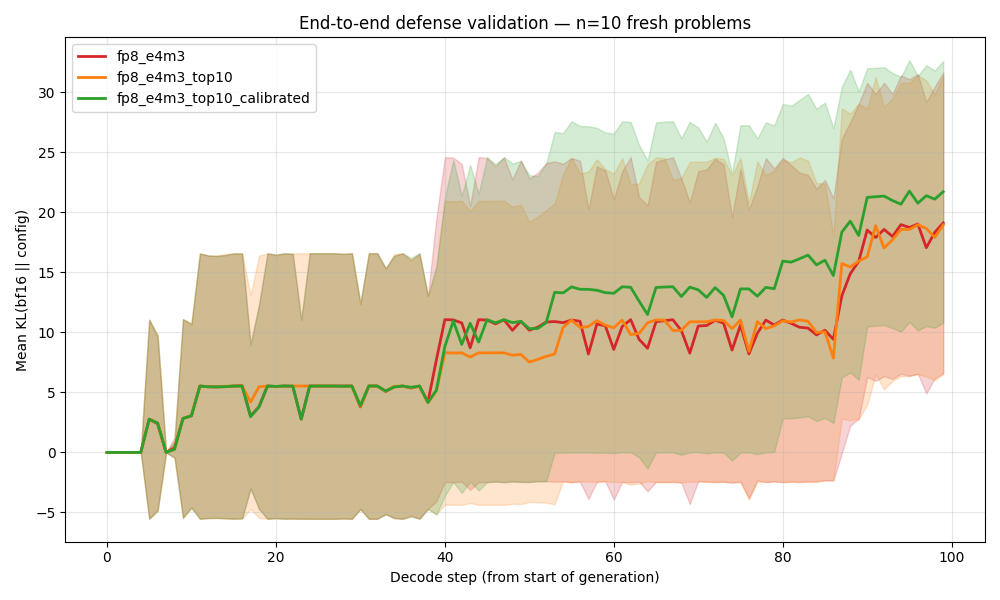
\includegraphics[width=0.85\textwidth]{figures/fig_defense_ar.png}
\caption{Средняя logit KL между bf16 и fp8 траекториями как функция шага декодирования AR-генерации (10 свежих задач MATH-500, max 100 токенов). Лабораторное $-15~\%$ снижение attention KL транслируется в $-2{,}4~\%$ снижение logit KL; SmoothQuant-стиль калиброванной защиты на основе prefill K дополнительно ухудшает результат.}
\label{fig:defense_ar}
\end{figure}

\begin{table}[H]
\centering
\caption{End-to-end AR-валидация защиты (10 задач, 100 токенов, greedy).}
\label{tab:ar_gap}
\small
\begin{tabular}{lccc}
\toprule
Метрика & fp8 baseline & top-10 per-step & top-10 calibrated \\
\midrule
Mean first divergence step & 57{,}5  & 58{,}9 (+1{,}4) & 52{,}4 ($-$5{,}1) \\
Token agreement @100       & 0{,}658 & 0{,}668 (+0{,}010) & 0{,}600 ($-$0{,}058) \\
Mean logit KL              & 8{,}749 & 8{,}539 ($-$2{,}4~\%) & 10{,}329 (+18{,}1~\%) \\
\bottomrule
\end{tabular}
\end{table}

Причины: (а) identity outlier-каналов нестабильна на одно-токеновых декод-шагах; (б) восстановление K-ошибки в одной позиции не пропагирует через каскад softmax $\to$ hidden $\to$ logit в compounding AR-режиме. Защита, применённая в TF/scoring рабочих нагрузках, по-прежнему даёт паспортные $-34~\%$ K-error и $-15~\%$ attention KL.

\subsection{Отрицательный результат: failure prediction}

Гипотеза о том, что ранний участок KL (первые 30--200 позиций) предсказывает финальное расхождение, не подтвердилась. LOO-CV AUC логистической регрессии для fp8\_e4m3: 0{,}424 ($n=30$), 0{,}394 ($n=50$), 0{,}506 ($n=100$), 0{,}573 ($n=200$). Для fp8\_e5m2 результаты ещё ниже, до 0{,}283. Ранний KL --- не надёжный детектор collapse'а.

% ============== ОБСУЖДЕНИЕ ==============
\section{Обсуждение}

\subsection{Что переносится между моделями}

\textbf{Универсальные claim'ы} (подтверждены на 4 моделях):
\begin{enumerate}[label=\arabic*.,leftmargin=*]
\item Magnitude relative K-error определяется только форматом квантизации, не архитектурой модели.
\item HQQ всегда обеспечивает 4--5$\times$ более равномерное распределение шума по каналам, чем FP8.
\item Направление эффекта per-channel защиты: для FP8 \textit{помогает} (на любой модели с concentration $>20~\%$), для HQQ практически нейтрально.
\end{enumerate}

\textbf{Model-specific claim'ы}:
\begin{enumerate}[label=\arabic*.,leftmargin=*]
\item Точная величина концентрации (52~\% на Qwen3-1.7B, 17~\% на SmolLM2).
\item Величина recovery защиты (масштабируется линейно с концентрацией).
\item Конкретные victim/safe слои (L0, L5, L23--L27 --- только Qwen3-1.7B).
\item Характеристическое время $\tau$ траектории KL.
\end{enumerate}

\subsection{Ограничения}

\begin{enumerate}[label=\arabic*.,leftmargin=*]
\item \textbf{Одна базовая модель} для глубокого анализа (Qwen3-1.7B). Кросс-валидация проведена на $n=5$--20 для других моделей.
\item \textbf{CPU-симуляция}, не GPU-ядро. Bit-точное сравнение с vLLM проведено только на первых 10 декод-токенах задачи 0.
\item \textbf{$N = 30$ задач для HQQ ablation} --- $\sim$300 мс/вызов делает $n=80$ неосуществимым в бюджете CPU.
\item \textbf{Greedy и $T=0{,}6$} только, без sweep по температуре.
\item \textbf{Отсутствует прямое сравнение с SmoothQuant и AWQ} --- они требуют другой инфраструктуры.
\end{enumerate}

\subsection{Дальнейшая работа}

\begin{enumerate}[label=\arabic*.,leftmargin=*]
\item Динамическая идентификация outlier-каналов, адаптированная к compounding AR-дрифту.
\item Расширенный protection set (top-30, top-50) для крупных моделей с разбавленной концентрацией.
\item Cross-family layer-importance ranking --- какие слои universally критичны.
\item Тест на multi-modal моделях (Qwen-VL, LLaVA) --- может ли видеоконтекст изменить outlier-структуру.
\item Bit-точное сравнение с vLLM на полном datasets.
\end{enumerate}

% ============== ЗАКЛЮЧЕНИЕ ==============
\section{Заключение}

В работе предложен и реализован первый pipeline механистического CPU-анализа KV-кеш-квантизации в reasoning-моделях. На примере Qwen3-1.7B и трёх дополнительных моделей показано:

\begin{enumerate}[label=\arabic*.,leftmargin=*]
\item Шум FP8-квантизации структурно концентрирован: 10 каналов из 1024 (1~\%) несут более половины шума на Qwen-семействе. На Llama-derived моделях концентрация значительно меньше (17~\% против 52~\%).
\item Защита top-10 outlier-каналов в bf16 восстанавливает 29--34~\% K-ошибки и 15~\% attention shift в лабораторной TF-метрике на Qwen-моделях. На Llama-derived моделях восстановление пропорционально меньше ($\sim$9~\%).
\item HQQ-формат уже включает outlier-aware квантизацию на уровне per-group scale; per-channel защита для него практически нейтральна.
\item В end-to-end AR-генерации лабораторное $-15~\%$ снижение attention KL транслируется только в $-2{,}4~\%$ снижение logit KL. SmoothQuant-стиль калиброванной защиты в AR ухудшает результат.
\item Раннюю KL-траекторию нельзя использовать как детектор финального расхождения (AUC $<$ 0{,}6).
\end{enumerate}

Полный pipeline захвата (\textasciitilde 80 ГБ raw артефактов), скрипты анализа и кросс-модельная валидация выложены в открытый доступ. Результаты служат основой для дальнейших мехинтерп-исследований квантизации языковых моделей и для калибровки production inference stack'ов.

% ============== ЛИТЕРАТУРА ==============
\renewcommand{\refname}{Список использованных источников}
\begin{thebibliography}{9}

\bibitem{micikevicius2022}
Micikevicius P., Stosic D., Burgess N. \textit{и др.}
FP8 Formats for Deep Learning.
arXiv:2209.05433, 2022.

\bibitem{badri2023}
Badri H., Shaji A.
Half-Quadratic Quantization of Large Machine Learning Models.
Mobius Labs Technical Blog, 2023.

\bibitem{kwon2023}
Kwon W., Li Z., Zhuang S. \textit{и др.}
Efficient Memory Management for Large Language Model Serving with PagedAttention~//
Proceedings of SOSP. --- 2023.

\bibitem{xiao2023smoothquant}
Xiao G., Lin J., Seznec M. \textit{и др.}
SmoothQuant: Accurate and Efficient Post-Training Quantization for Large Language Models~//
Proceedings of ICML. --- 2023.

\bibitem{lin2024awq}
Lin J., Tang J., Tang H. \textit{и др.}
AWQ: Activation-aware Weight Quantization for LLM Compression and Acceleration~//
Proceedings of MLSys. --- 2024.

\bibitem{olah2020zoom}
Olah C., Cammarata N., Schubert L. \textit{и др.}
Zoom In: An Introduction to Circuits~//
Distill. --- 2020.

\bibitem{templeton2024scaling}
Templeton A., Conerly T., Marcus J. \textit{и др.}
Scaling Monosemanticity: Extracting Interpretable Features from Claude 3 Sonnet.
Anthropic Technical Report, 2024.

\bibitem{qwen3report}
Qwen Team.
Qwen3 Technical Report.
Alibaba Cloud, 2025.

\bibitem{deepseekr1}
DeepSeek-AI.
DeepSeek-R1: Incentivizing Reasoning Capability in LLMs via Reinforcement Learning.
arXiv:2501.12948, 2025.

\end{thebibliography}

\end{document}
